\documentclass{article}
\usepackage{enumitem}
\usepackage{graphicx}
\usepackage{adjustbox}
\usepackage{amsmath}
\usepackage[margin=3cm]{geometry}
\usepackage{dirtree}
\usepackage{float}
\usepackage{listings}

\graphicspath{ {./images/} }

\begin{document}
\title{NotArmLeg documentation}
\author{William Kelly, Alex Thomas, Charles, Luke} 
\maketitle{}

\begin{center}
    \centering
    
\includegraphics[width=0.9\textwidth]{armnotleg}
\end{center}
\newpage

\section{Introduction}
This project is designed to train users to not click on spam emails.

They will add they're email using the website and choose the maximum number of emails they wish to have sent per month and then we will send them fake spam. On this fake spam is a link which if pressed they get redirected to our website which will display information about the features of the email that suggests that it is spam. This is designed to educate the user and hopefully mitigate them accidentally clicking on spam emails.

\section{Module interaction}
The project consists of 4 modules:
\begin{itemize}
    \item Web server
    \item Database
    \item Spam repo
    \item Email server
    \item Repository generator

\end{itemize}
The web server uses flask for its backend. We are using mySQL for the data base. The spam repo is is a file server with a defined hirearchy for storing spam emails and finally the email server is written in python.

\section{Repo hirearchy}

\begin{figure}[H]
\dirtree{%
    .1 repo.
    .2 spamrepo.
    .3 mail1.
    .4 subject.txt.
    .4 mail.txt.
    .4 features.json.
    .3 mail2.
    .4 subject.txt.
    .4 mail.txt.
    .4 features.json.
    .3 etc.
    .2 featureRepo.
    .3 feature1.
    .4 body.txt.
    .4 header.txt.
    .4 image.jpg.
    .3 feature2.
    .4 body.txt.
    .4 header.txt.
    .4 image.jpg.
    .3 etc.
}
\caption{Repository hirearchy for spam emails}
\end{figure}

The spam repo is used to store all the emails that would be sent to the users. Inside this directory exists a mail.txt file that stores the html of the email. The features.json file contains metadata on the email. This metadata is information that says what about the email indicates that it is spam. Features can be found inside the feature repo. Each feature has a body, header allong with an image that is fetched once a link inside a spam email has been pressed. This can then be displayed on the webpage as the information used to educate the user.

\begin{lstlisting}[frame=single, caption={features.json}]
{
    "features":[
        {
            "name":"funkyAddress",
            "id":"funkyAddress",
            "repository","repourl/telloffsite/featurerepo"
        },
        {
            "name":"funkySpelling",
            "id":"funkySpelling",
            "repository","repourl/telloffsite/featurerepo"
        }
    ]
}
\end{lstlisting}

\section{MySQL database}
\begin{center}
    \centering
    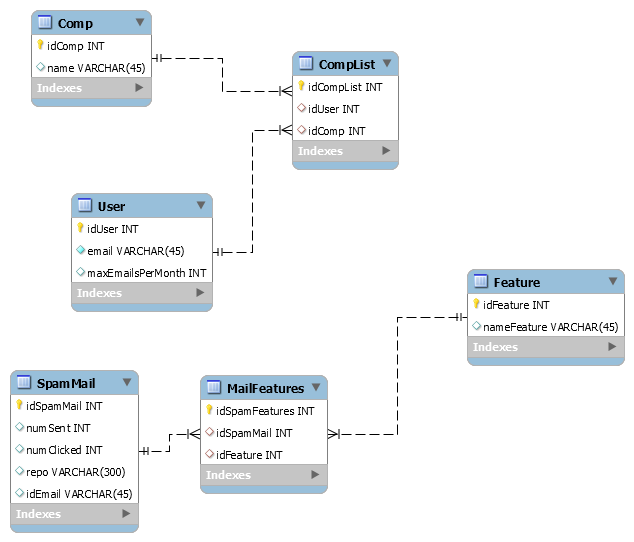
\includegraphics[width=0.8\textwidth]{database}
    \begin{figure}[H]
        \caption{MySQL database layout}
    \end{figure}
\end{center}
\end{document}

